\clearpage
\section{نطاقات البريد الإلكتروني}
\label{sec:settings-feature-email-domains}

النطاق هو الجزء الذي يلي الرمز @ في عنوان البريد، وهو يمثل اسم مؤسستك على الإنترنت. تسجله هنا لتثبت أنك تملكه، ثم تنشئ عليه صناديق بريد لأعضاء المؤسسة. وتحتاج إلى هذه الصفحة مرة واحدة عند إضافة نطاق، ثم تعود إليها إذا ظهرت مشكلة في البريد.

سجلات \en{DNS} هي أسطر قصيرة تضيفها في موقع الجهة التي اشتريت منها النطاق، فتخبر خدمات الإنترنت أين تذهب رسائلك ومن يحق له الإرسال باسمك. ولا يفتح هذه الصفحة إلا مالك المؤسسة.

\begin{rcnote}[مثال: شركة الأفق]
يكتب مسؤول النظام، وهو مالك المؤسسة في الأفق، نطاق الشركة عند ①، ويضغط ②، ثم يطلب من الشركة التي تدير النطاق إضافة السجلات الظاهرة. وبعد إضافتها يضغط ④، فتصبح الحالة عند ③ «نشط»، ويمكن إنشاء بريد لعمر حداد على هذا النطاق.
\end{rcnote}
\begin{figure}[H]
\centering
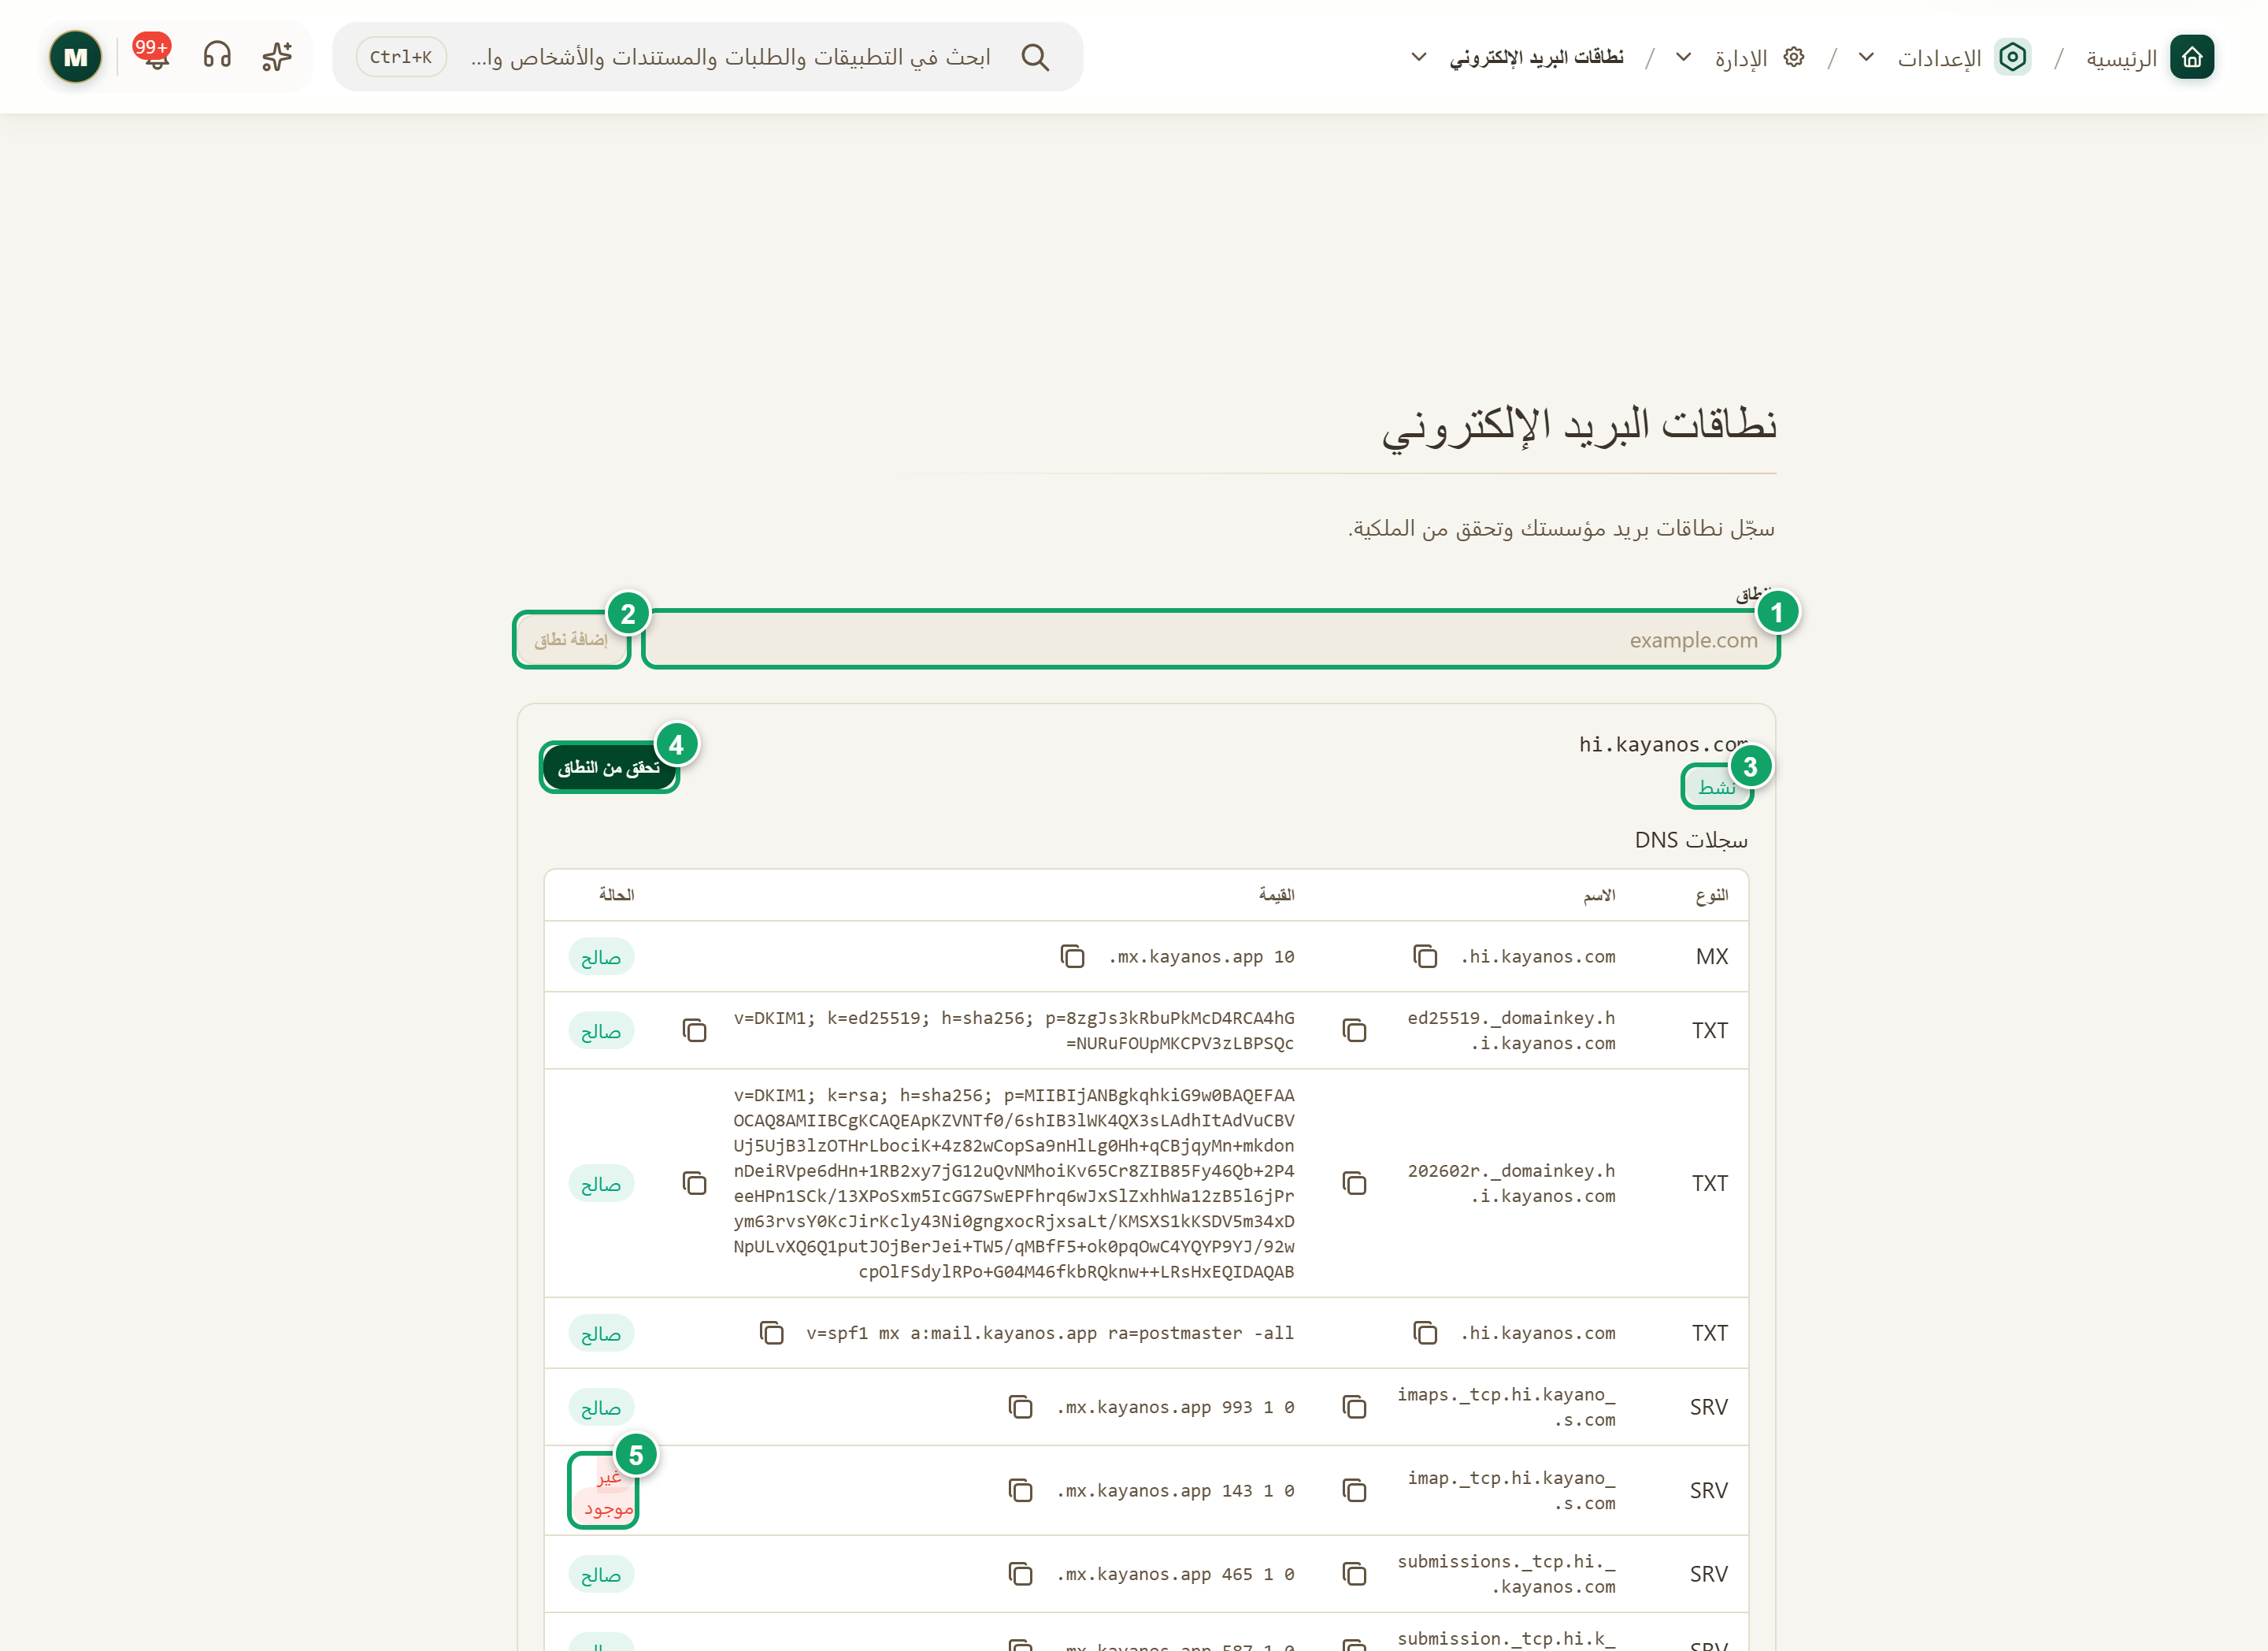
\includegraphics[width=0.95\linewidth,height=0.72\textheight,keepaspectratio]{figures/screens/ch08-email-domains-ar.png}
\caption{نطاق نشط وسجلات DNS}
\label{fig:settings-email-domains}
\shotnote{تعرض الصورة نطاق اختبار مفعّلاً وبداية جدول سجلاته، وفيها سجل مفقود رغم أن النطاق نشط؛ فالحالتان مختلفتان. توقفت الصورة قبل نهاية الجدول لأن آخر صف يحمل قيمة تحقق خاصة لا يصح نشرها. ① حقل «النطاق». ② «إضافة نطاق»: يبقى معطلاً حتى تكتب النطاق. ③ حالة النطاق. ④ «تحقق من النطاق». ⑤ حالة السجل: «غير موجود» يعني أن السجل لم يُعثر عليه.}
\end{figure}

\begin{figure}[H]
\centering
\begin{tikzpicture}[node distance=0.5cm]
\node[stepBox] (a) {\RL{إضافة النطاق في هذه الصفحة}};
\node[stepBox,below=of a] (b) {\RL{نسخ سجلات \en{DNS} إلى مزوّد النطاق}};
\node[stepBox,below=of b] (c) {\RL{الضغط على «تحقق من النطاق»}};
\node[stepBox,below=of c] (d) {\RL{تصبح حالة النطاق «نشط»}};
\node[stepBox,below=of d] (e) {\RL{إنشاء صناديق البريد على النطاق}};
\draw[flowsTo] (a) -- (b);
\draw[flowsTo] (b) -- (c);
\draw[flowsTo] (c) -- (d);
\draw[flowsTo] (d) -- (e);
\end{tikzpicture}
\rclegend
\caption{مراحل تفعيل نطاق البريد}
\label{fig:settings-email-domains-flow}
\shotnote{لا تنتقل هذه المراحل وحدها؛ فكل مرحلة إجراء تقوم به أنت، ولا يكتمل التحقق قبل أن تصبح السجلات ظاهرة على الإنترنت. لذلك إذا ضغطت زر التحقق مبكراً فأصبحت الحالة «خطأ»، فانتظر قليلاً ثم أعد المحاولة.}
\end{figure}

\begin{table}[H]
\centering
\caption{ماذا تقرأ في نطاقات البريد؟}
\label{tab:settings-email-domains-fields}
\begin{tabularx}{\linewidth}{R{4.2cm} Y}
\rcHeaderRow
\thh{البيان} & \thh{ماذا يعني؟}\\
«النطاق» & النطاق الأساسي الذي تريد استخدامه للبريد. لا يمكن تسجيله إذا كان مسجلاً لمؤسسة أخرى.\\
حالة النطاق & «قيد الانتظار» قبل نجاح التحقق، و«نشط» بعد اكتماله، و«خطأ» إذا فشل. وتظهر «تم التحقق» لحظة انتقاله إلى «نشط».\\
«سجلات \en{DNS}» & لكل سجل «النوع» و«الاسم» و«القيمة» و«الحالة»، وبجوار الاسم والقيمة زر للنسخ.\\
حالة السجل & «صالح»، أو «غير مطابق» إذا اختلفت القيمة، أو «غير موجود»، أو «غير معروف».\\
«حذف النطاق» & يظهر فقط عندما تكون الحالة «قيد الانتظار» أو «خطأ».\\
\end{tabularx}
\end{table}

\begin{enumerate}
\item افتح «الإعدادات»، ثم «نطاقات البريد الإلكتروني».
\item اكتب النطاق في حقل «النطاق»، ثم اضغط «إضافة نطاق».
\item انسخ قيمة كل سجل بزر النسخ، وأضفه عند مزوّد النطاق.
\item اضغط «تحقق من النطاق» بعد إضافة السجلات.
\item راجع حالة النطاق، ثم راجع حالة كل سجل في الجدول.
\end{enumerate}

\textbf{تحقق:} تظهر حالة «نشط» ورسالة نجاح. يفحص الزر سجل إثبات الملكية فقط، لذلك راجع بقية السجلات بنفسك، وصحّح ما حالته «غير موجود» أو «غير مطابق» إذا تعطل الإرسال أو الاستقبال. وانتبه إلى أن إعادة التحقق بعد حذف سجل الملكية تحوّل الحالة إلى «خطأ».

\clearpage
\section{توقيعات البريد الإلكتروني}
\label{sec:settings-feature-email-signatures}

التوقيع هو الجزء الذي يظهر في نهاية الرسالة ويحمل اسم المرسل ومنصبه وطرق التواصل معه. تصمم هنا قالباً واحداً تملؤه بيانات كل عضو تلقائياً، فتتوحد صورة رسائل المؤسسة دون أن يكتب كل عضو توقيعه. وإخلاء المسؤولية نص قانوني مشترك يُضاف إلى الرسائل الصادرة.

استخدم هذه الصفحة عند اعتماد توقيع للمؤسسة أو تغيير هويتها. لا يديرها إلا مالك المؤسسة، ويرى غيره رسالة توضح ذلك. أما كل عضو فيدير توقيعاته الشخصية من «إدارة التوقيعات…» عند كتابة رسالة، ما لم يكن توقيع المؤسسة إلزامياً عليه.

\begin{rcnote}[مثال: شركة الأفق]
ينشئ مسؤول النظام قالباً باسم الأفق عند ② وينشره، ثم يضيف قاعدة تجعله إلزامياً على الجميع. وعندما يرسل عمر حداد رسالة جديدة يظهر اسمه ومنصبه تلقائياً، بينما تكشف البطاقة عند ④ الأعضاء الذين تنقصهم بيانات.
\end{rcnote}
\begin{figure}[H]
\centering
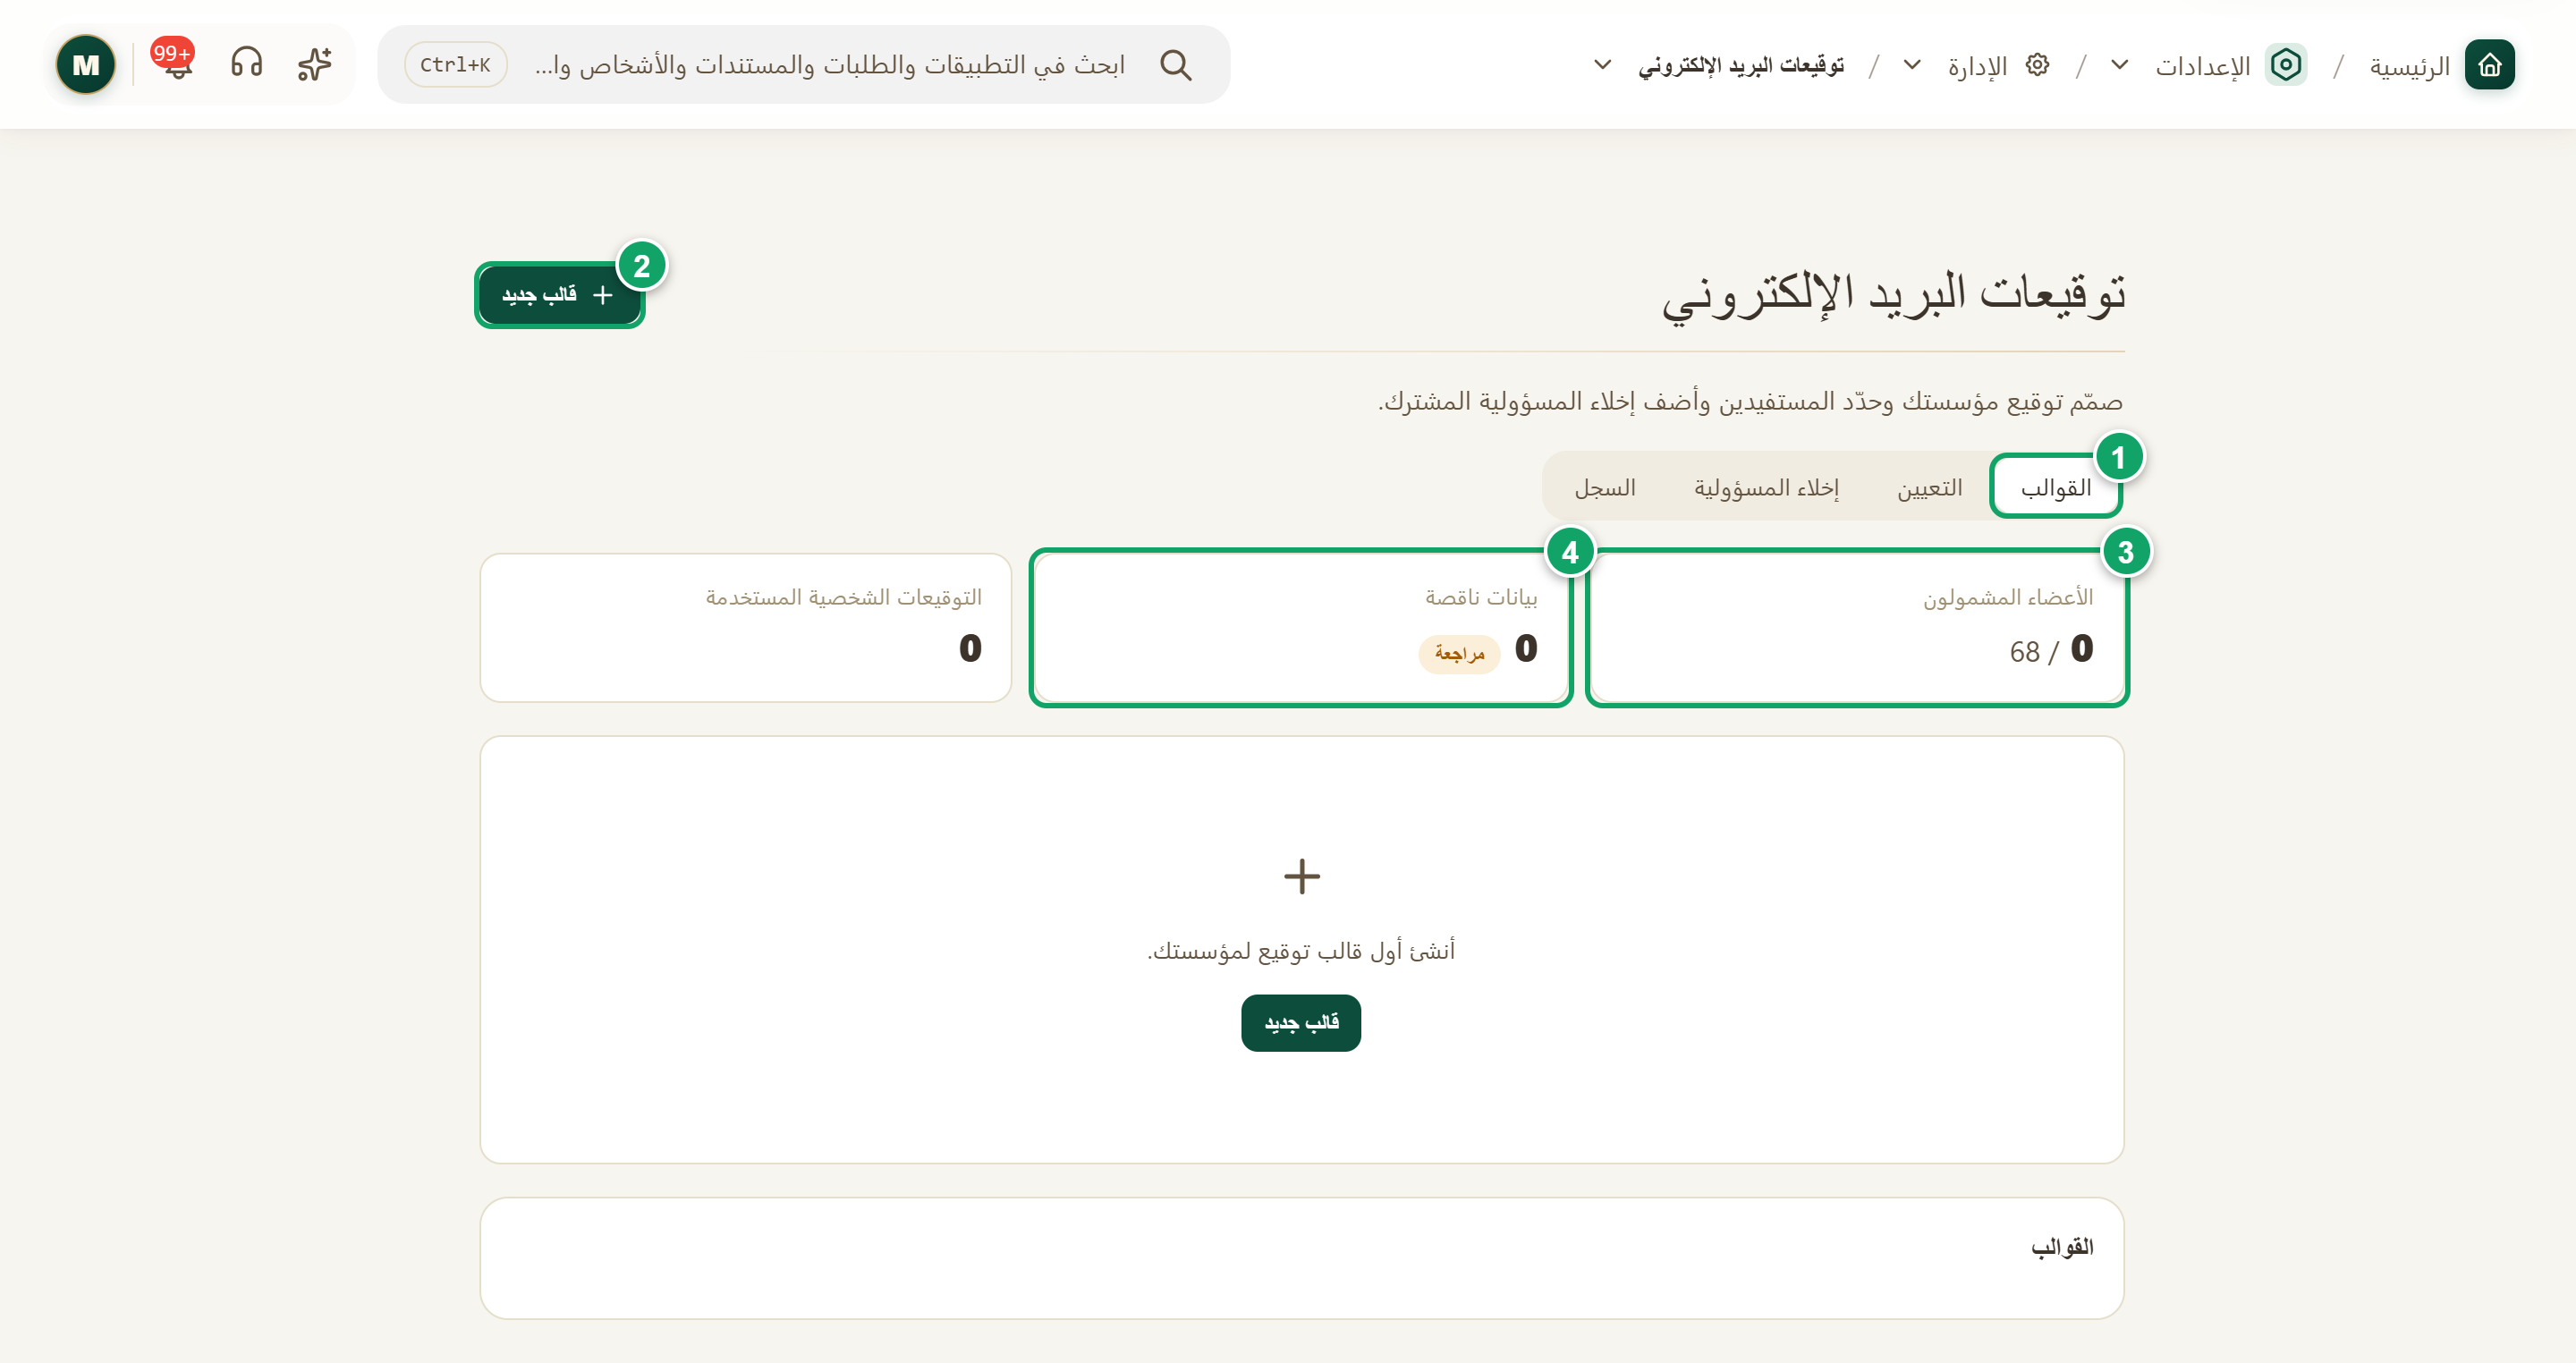
\includegraphics[width=0.95\linewidth,height=0.72\textheight,keepaspectratio]{figures/screens/ch08-email-signatures-ar.png}
\caption{تبويب القوالب}
\label{fig:settings-email-signatures}
\shotnote{تعرض الصورة بداية العمل في مؤسسة الاختبار قبل إنشاء أي قالب، لذلك لا يشمل التوقيع أي عضو. تساعدك البطاقات على متابعة التغطية بعد النشر. ① «القوالب». ② «قالب جديد». ③ «الأعضاء المشمولون»: عدد الأعضاء الذين ينطبق عليهم توقيع من أصل جميع الأعضاء. ④ «بيانات ناقصة»: تفتح مراجعة الأعضاء الذين ينقصهم حقل.}
\end{figure}

\begin{figure}[H]
\centering
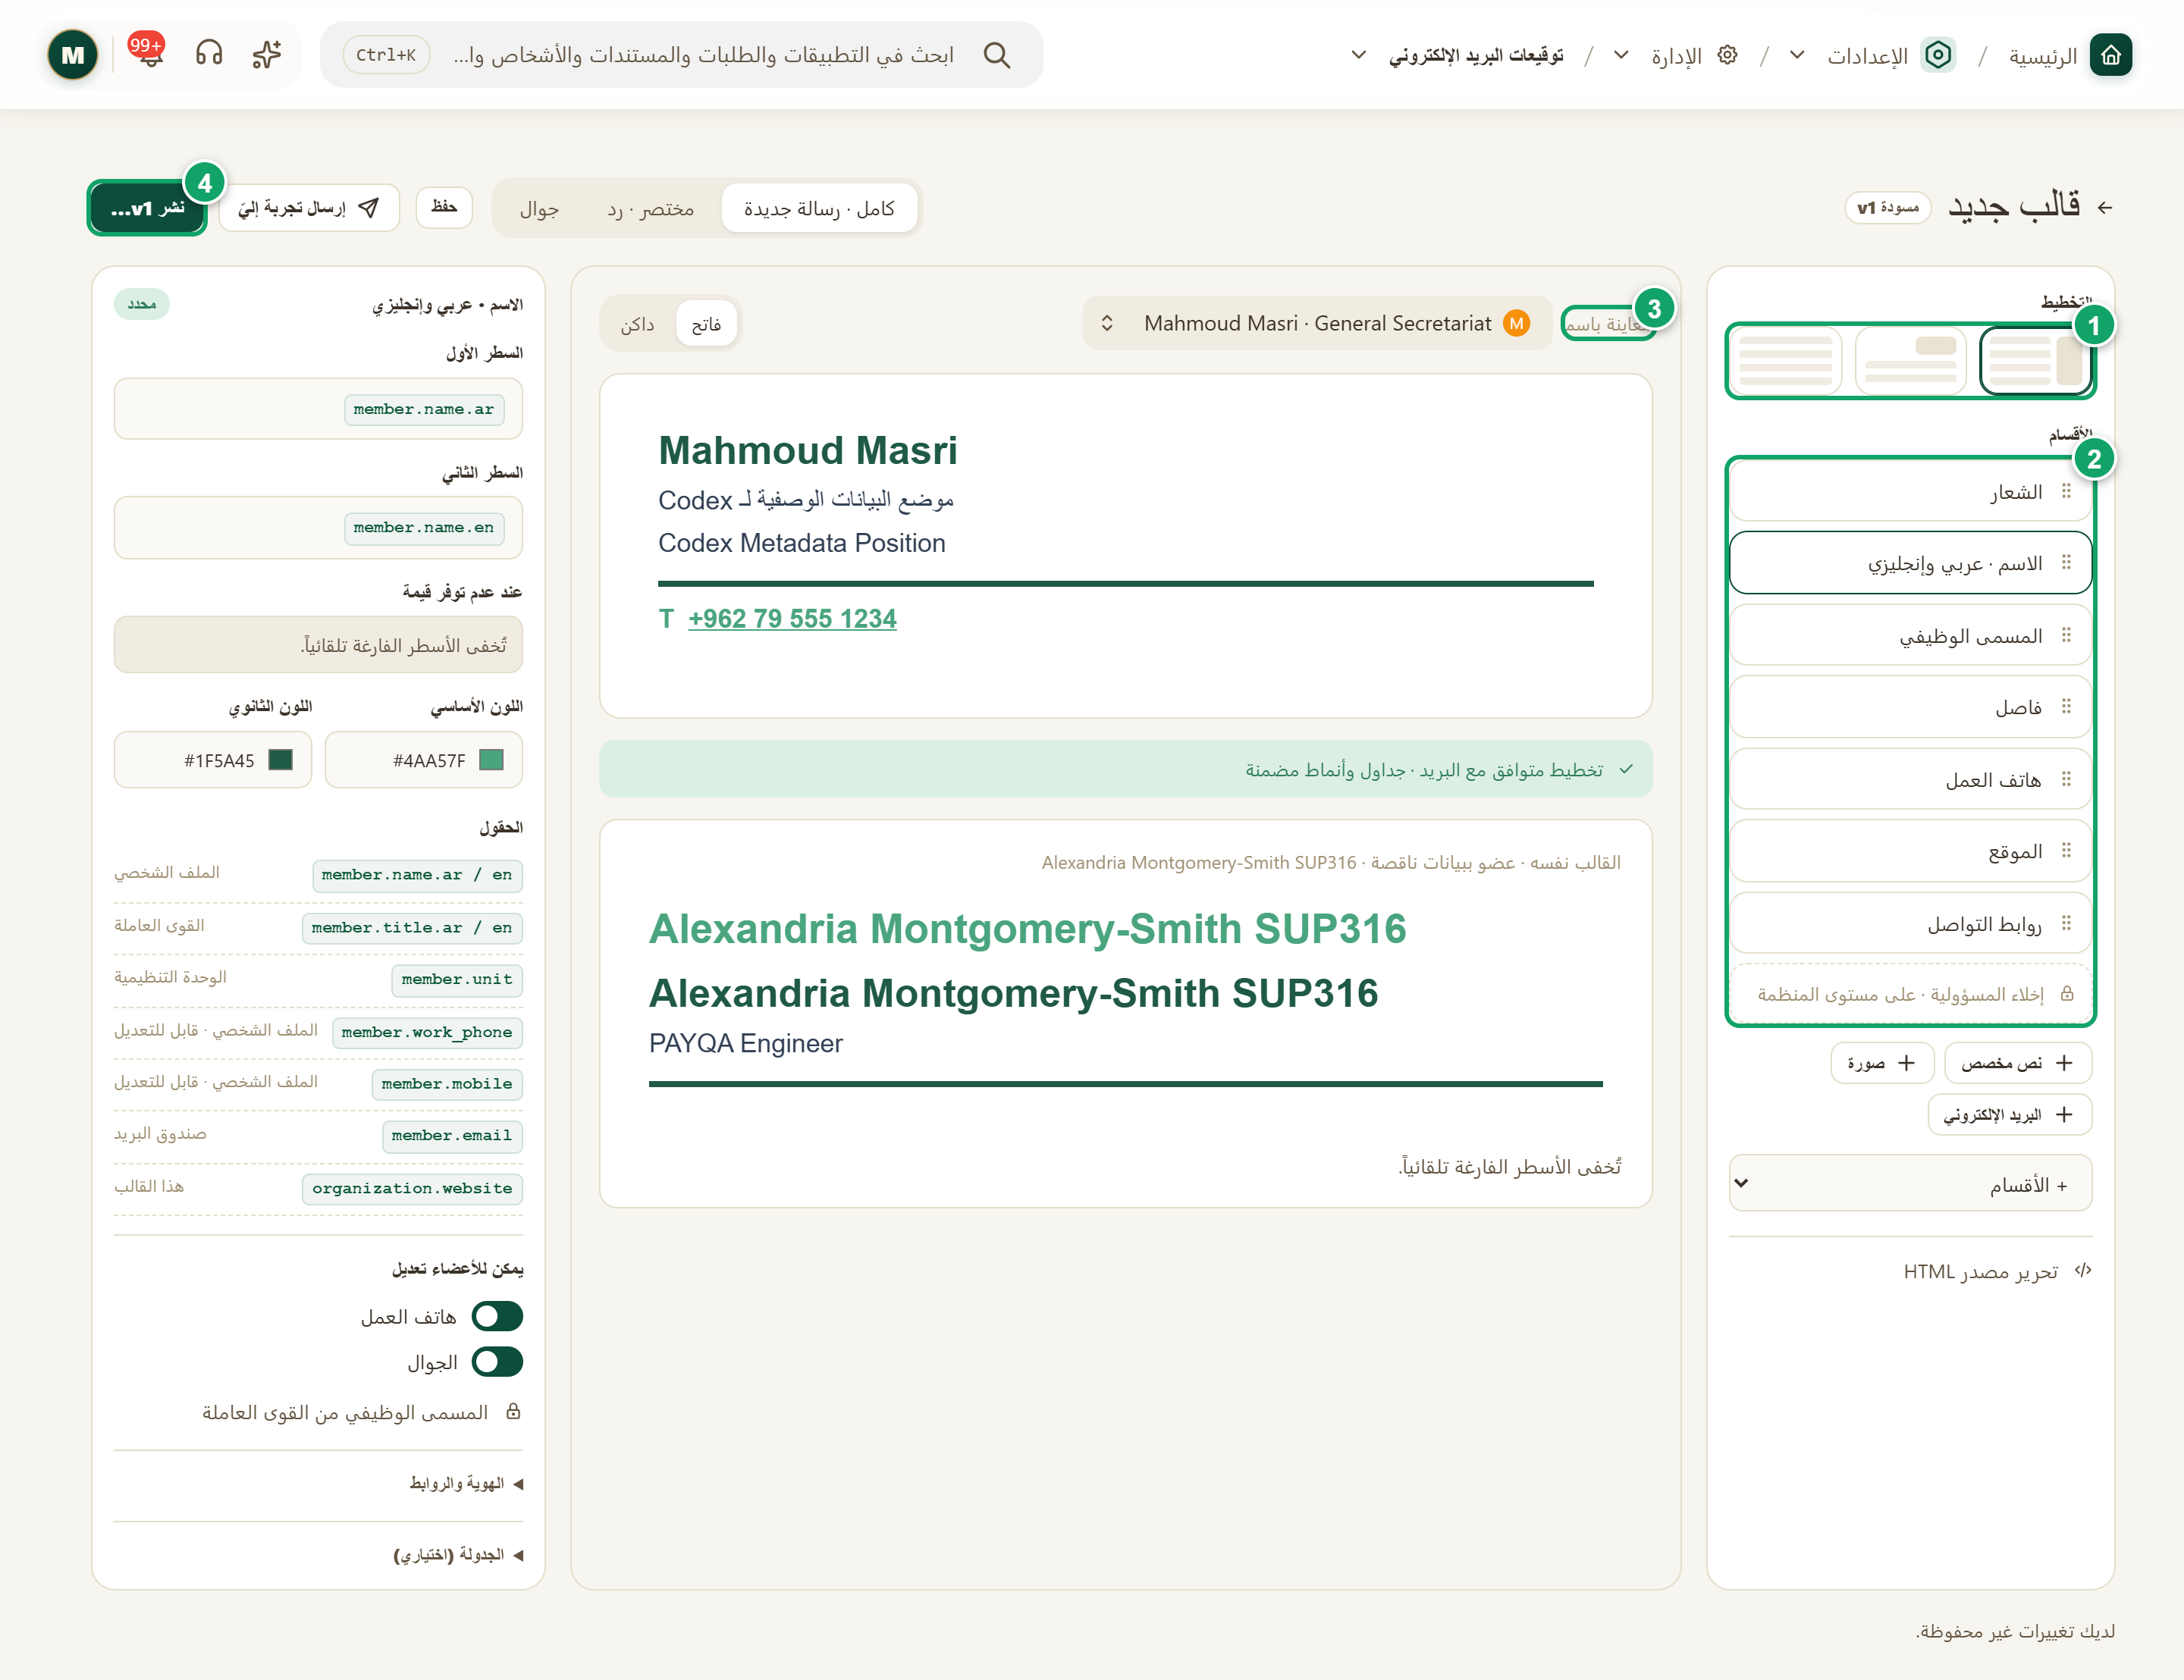
\includegraphics[width=0.95\linewidth,height=0.72\textheight,keepaspectratio]{figures/screens/ch08-email-signatures-designer-ar.png}
\caption{مصمم التوقيع}
\label{fig:settings-email-signatures-designer}
\shotnote{يفتح «قالب جديد» هذا المصمم، والقالب الظاهر تجريبي لم يُحفظ. تعرض المعاينة التوقيع ببيانات عضو من مؤسسة الاختبار، ثم ببيانات عضو آخر ناقصة، فترى أن الأسطر الفارغة تختفي تلقائياً. ① «التخطيط». ② «الأقسام»: ما يظهر في التوقيع وترتيبه. ③ «معاينة باسم»: لاختيار العضو الذي تعاين بياناته. ④ «نشر \en{v1}…»: يبدأ مراجعة البيانات قبل نشر الإصدار.}
\end{figure}

\begin{figure}[H]
\centering
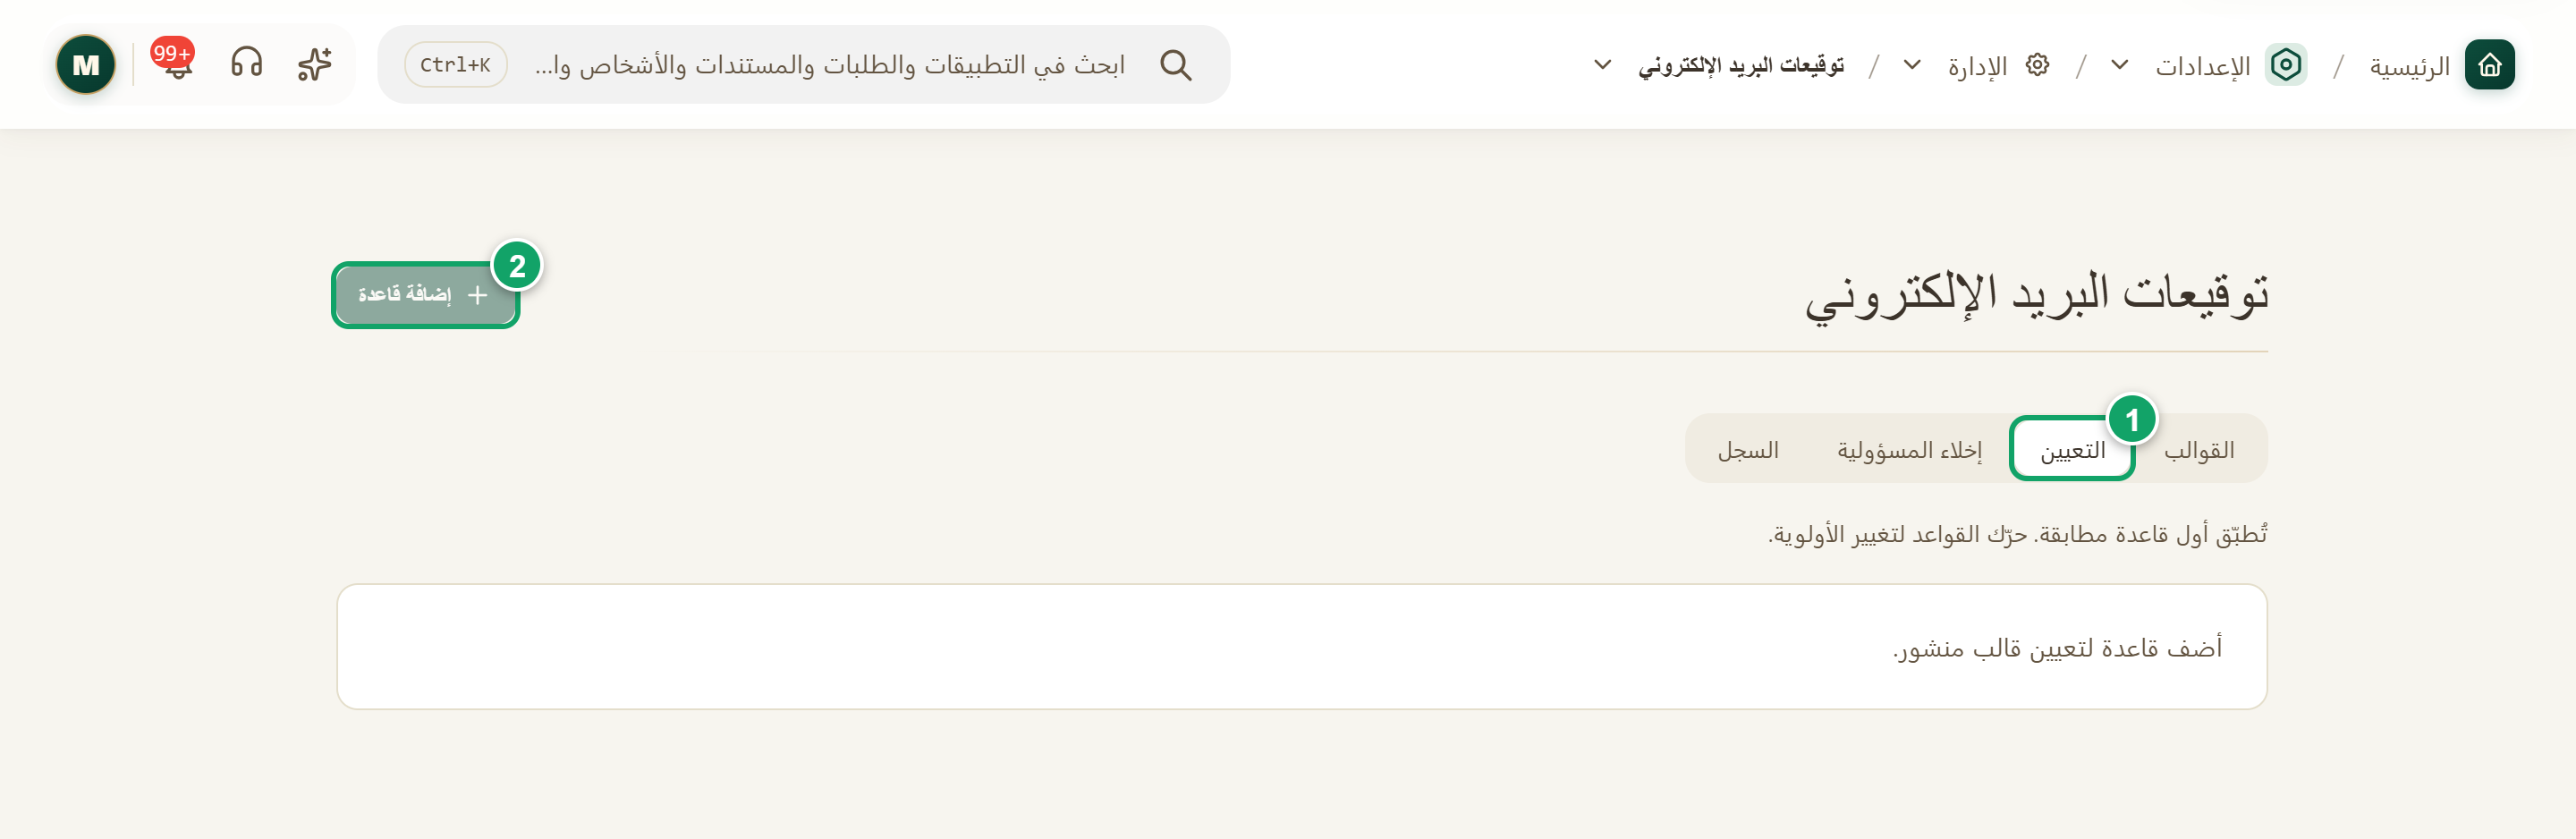
\includegraphics[width=0.95\linewidth,height=0.72\textheight,keepaspectratio]{figures/screens/ch08-email-signatures-assignment-ar.png}
\caption{تبويب التعيين}
\label{fig:settings-email-signatures-assignment}
\shotnote{يحدد التعيين من يستخدم كل قالب، ولا يصل القالب إلى الأعضاء دون قاعدة. الزر معطل في هذه الصورة لأن مؤسسة الاختبار لا تملك قالباً بعد. ① «التعيين». ② «إضافة قاعدة».}
\end{figure}

\begin{figure}[H]
\centering
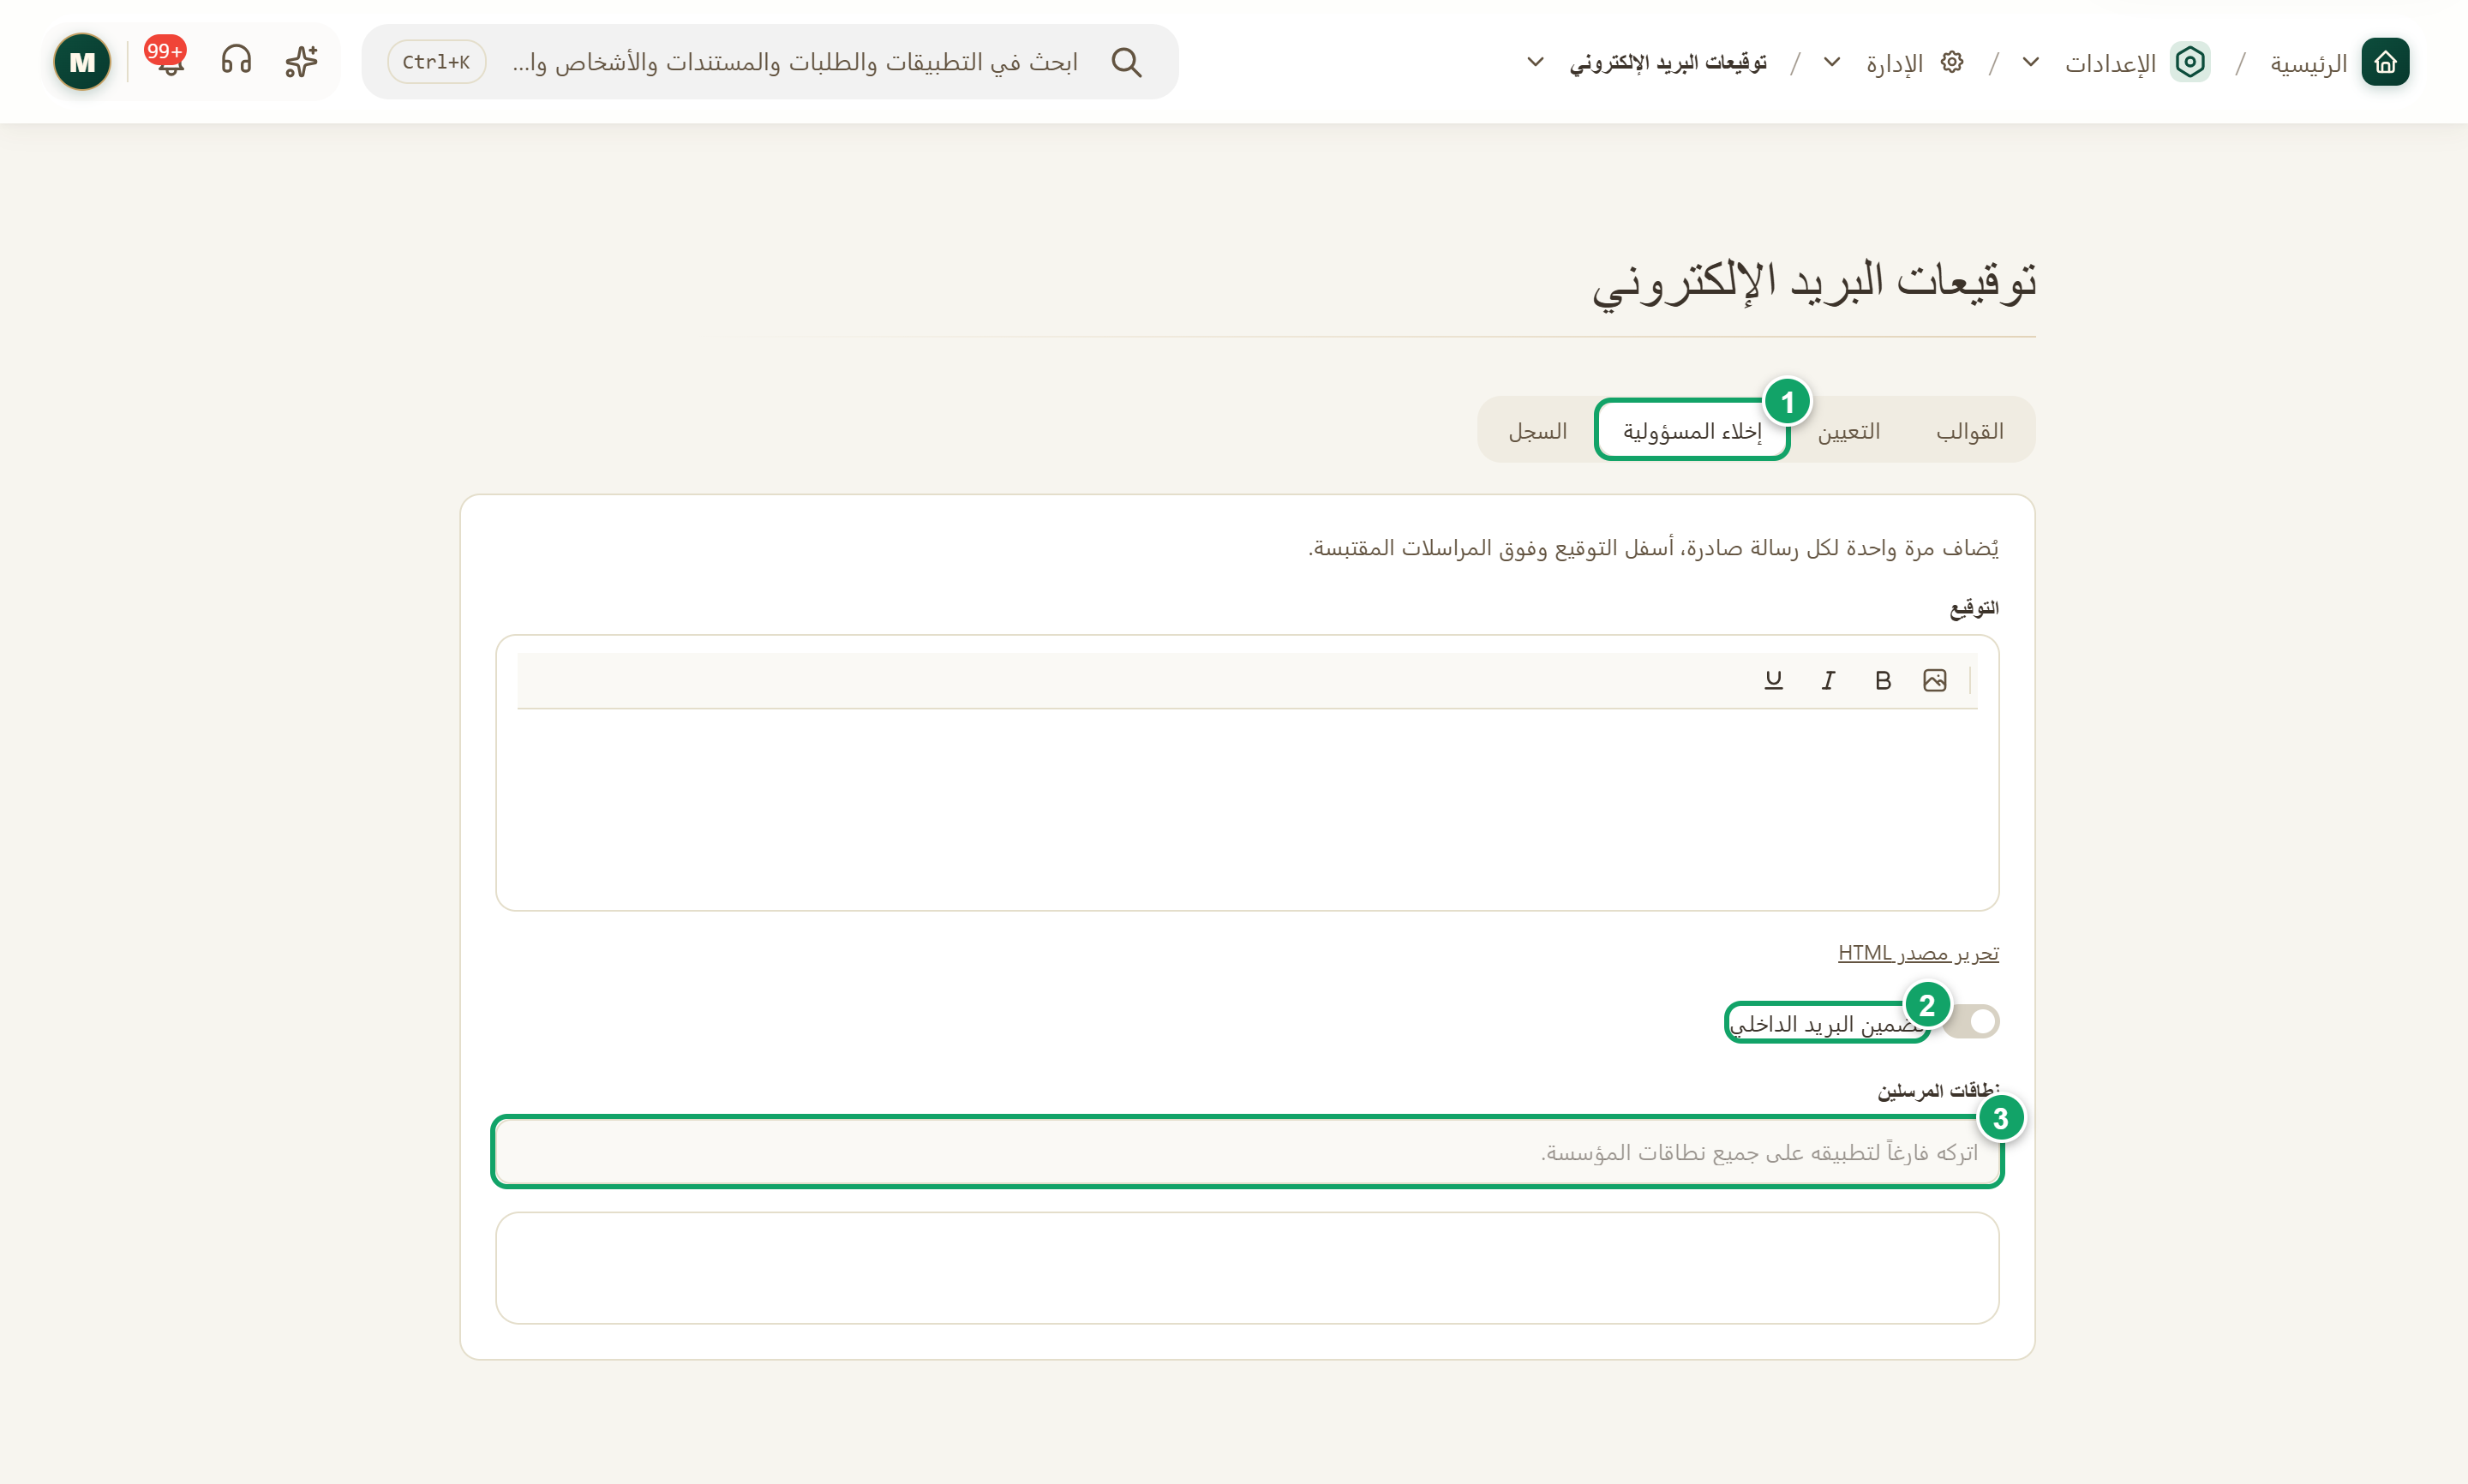
\includegraphics[width=0.95\linewidth,height=0.72\textheight,keepaspectratio]{figures/screens/ch08-email-signatures-disclaimer-ar.png}
\caption{تبويب إخلاء المسؤولية}
\label{fig:settings-email-signatures-disclaimer}
\shotnote{يُضاف هذا النص مرة واحدة لكل رسالة صادرة، أسفل التوقيع وفوق المراسلات المقتبسة، فلا يتكرر عند الردود. والنص فارغ في مؤسسة الاختبار. ① «إخلاء المسؤولية». ② «تضمين البريد الداخلي»: يضيف النص إلى الرسائل بين الأعضاء أيضاً. ③ حقل «نطاقات المرسلين»: اتركها فارغة ليشمل النص جميع نطاقات المؤسسة.}
\end{figure}

\begin{figure}[H]
\centering
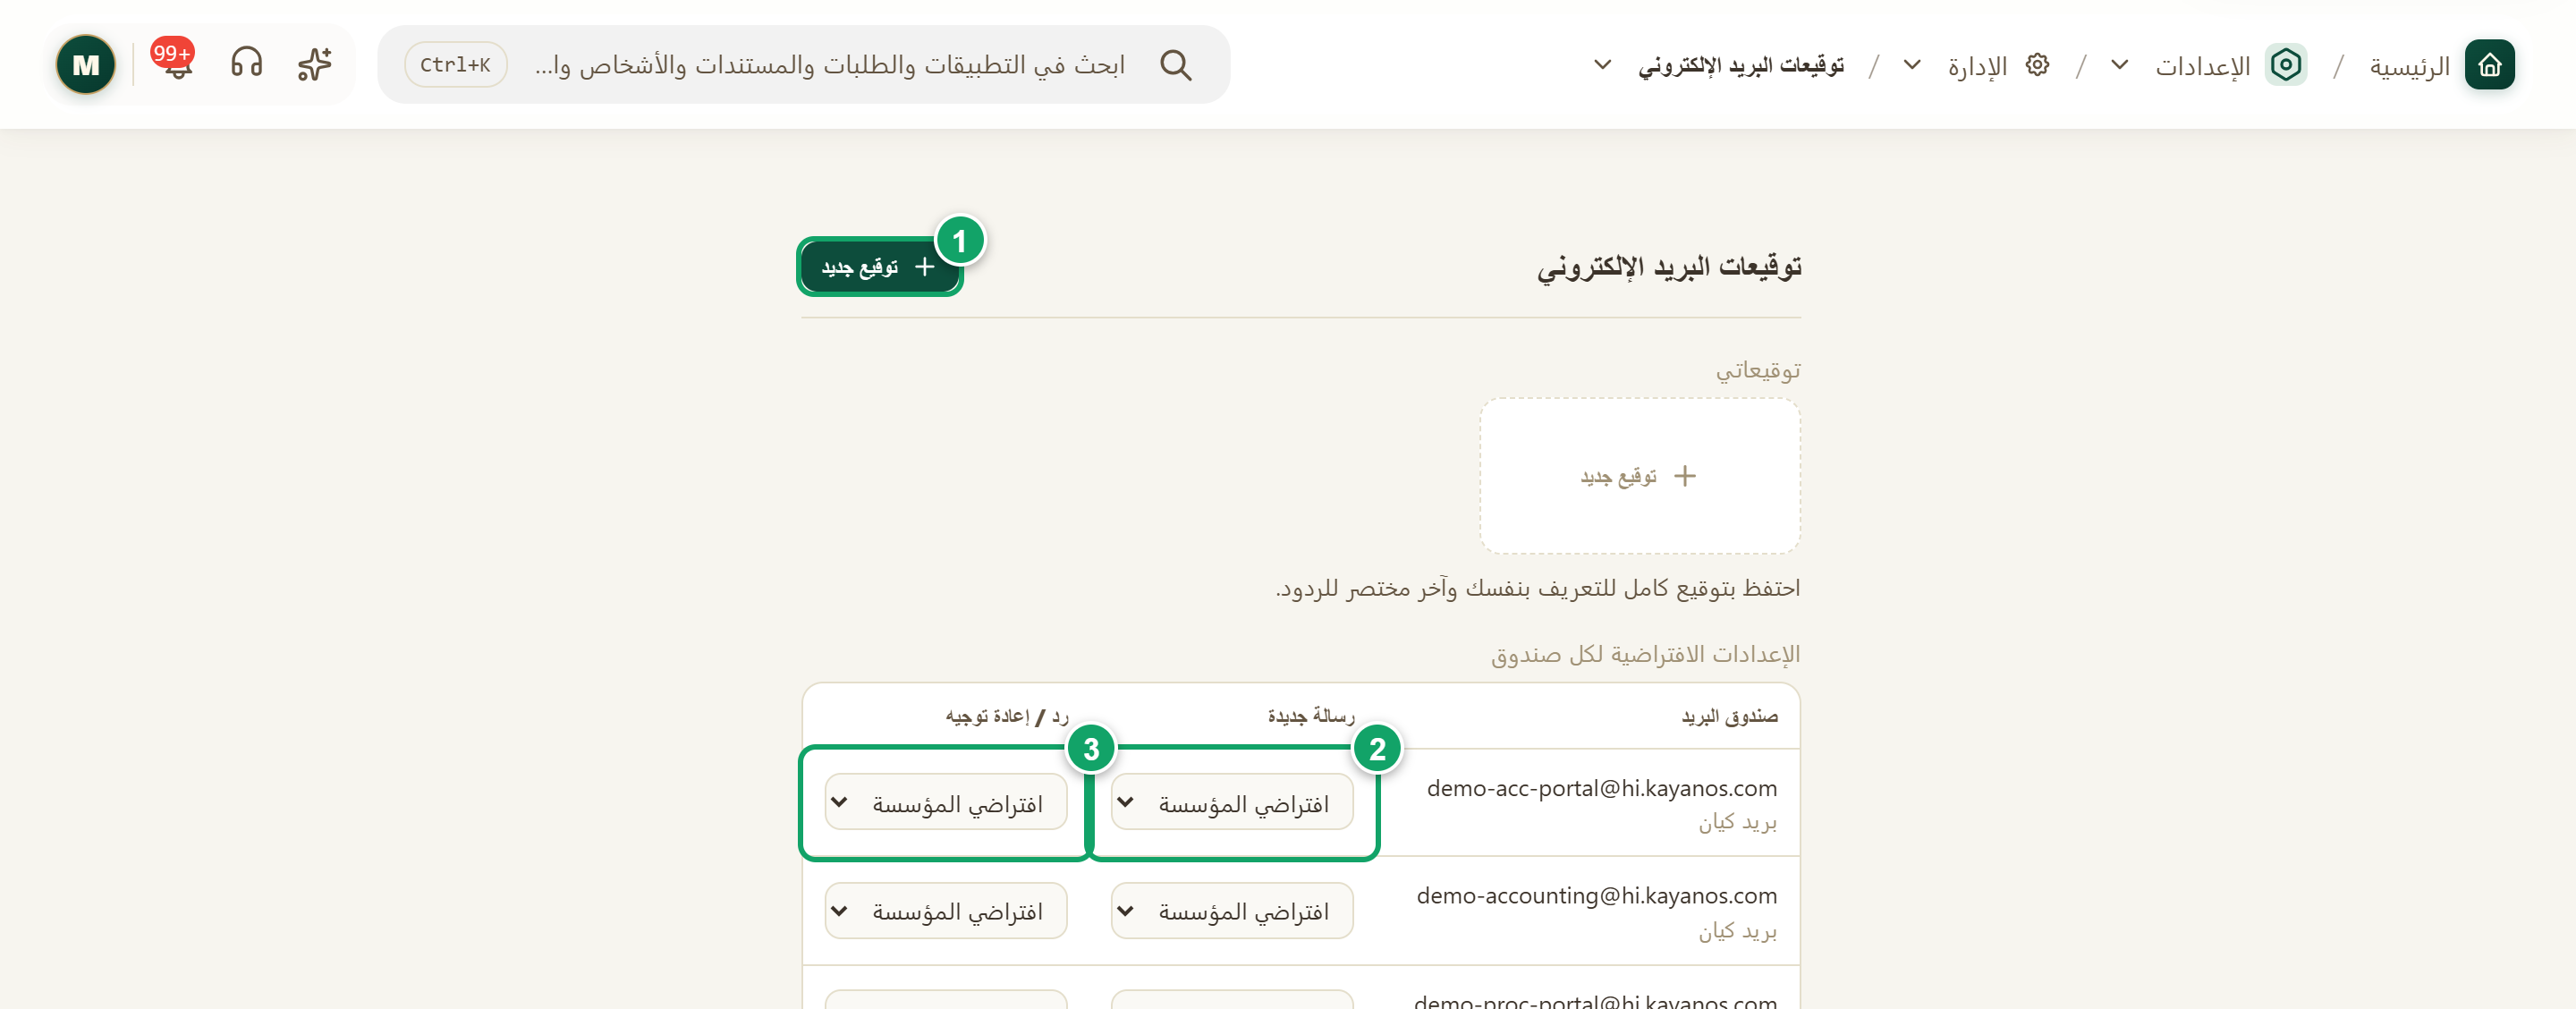
\includegraphics[width=0.95\linewidth,height=0.72\textheight,keepaspectratio]{figures/screens/ch08-email-signatures-personal-ar.png}
\caption{توقيعاتي}
\label{fig:settings-email-signatures-personal}
\shotnote{هذه هي الصفحة التي يراها العضو لنفسه، وتتيح له الاحتفاظ بتوقيع كامل وآخر مختصر للردود. يرتبط كل صف بصندوق بريد، فيمكن أن تختلف الإعدادات من صندوق إلى آخر. ① «توقيع جديد». ② التوقيع الافتراضي للرسائل الجديدة من هذا الصندوق. ③ التوقيع الافتراضي للردود وإعادة التوجيه.}
\end{figure}

\begin{table}[H]
\centering
\caption{ماذا تسجل في توقيعات البريد؟}
\label{tab:settings-email-signatures-fields}
\begin{tabularx}{\linewidth}{R{4.2cm} Y}
\rcHeaderRow
\thh{القسم} & \thh{ما الذي تسجله؟}\\
«القوالب» & الاسم، و«التخطيط»، و«الأقسام»، والألوان، و«الهوية والروابط»، و«الجدولة (اختياري)»، والحقول المسموح بتعديلها في «يمكن للأعضاء تعديل». ولكل قالب ثلاث نسخ: «كامل · رسالة جديدة» و«مختصر · رد» و«جوال».\\
«التعيين» & قواعد لها «تنطبق على» و«القالب» و«الوضع»، والنسخة المستخدمة للرسائل الجديدة والردود. تُطبَّق أول قاعدة مطابقة، فرتّبها بحسب الأولوية.\\
«الوضع» & «إلزامي»: يُضاف دائماً ولا يغيّره العضو. «افتراضي»: محدد مسبقاً ويمكن تغييره. «اختياري»: متاح في قائمة التوقيعات.\\
«إخلاء المسؤولية» & نص الإخلاء، و«تضمين البريد الداخلي»، و«نطاقات المرسلين».\\
«السجل» & الإصدارات المنشورة، مع «استعادة كإصدار جديد».\\
\end{tabularx}
\end{table}

\begin{enumerate}
\item افتح «الإعدادات»، ثم «توقيعات البريد الإلكتروني»، واضغط «قالب جديد».
\item اختر التخطيط والأقسام، ثم راجع المعاينة بأكثر من عضو.
\item اضغط «إرسال تجربة إليّ» إذا أردت رؤية التوقيع في صندوقك.
\item اضغط زر «نشر»، وراجع الأعضاء الذين تنقصهم بيانات، ثم أكمل النشر.
\item افتح «التعيين»، واضغط «إضافة قاعدة»، وحدد من تنطبق عليه القاعدة والقالب والوضع، ثم احفظ.
\end{enumerate}

\textbf{تحقق:} يتغير عدد «الأعضاء المشمولون» في تبويب «القوالب»، ويظهر الإصدار في «السجل». يُطبَّق الإصدار المنشور عند الإرسال التالي، بما في ذلك المسودات غير المرسلة، لذلك تأكد من الرسالة التالية التي يرسلها أحد الأعضاء.

\clearpage
\section{نطاقات الروابط القصيرة}
\label{sec:settings-feature-short-links}

الرابط القصير عنوان مختصر يصل إلى صفحة طويلة، ويسهل وضعه داخل رسالة. تتيح هذه الصفحة أن تحمل هذه الروابط اسم مؤسستك بدلاً من العنوان العام للمنصة، فيطمئن من يستلمها إلى مصدرها. والنطاق المخصص هنا عنوان فرعي تخصصه لهذه الروابط، مثل عنوان يبدأ بكلمة \en{links}.

هذه الصفحة اختيارية؛ فعندما لا يوجد نطاق نشط تُنشأ الروابط على عنوان المنصة الخاص بمؤسستك. ولا يديرها إلا مالك المؤسسة، ويرى غيره رسالة تطلب منه التواصل مع المالك. وتمر الإضافة بالمراحل نفسها المشروحة في صفحة نطاقات البريد (\ref{sec:settings-feature-email-domains}).

\begin{rcnote}[مثال: شركة الأفق]
يريد مسؤول النظام أن تحمل روابط رسائل الأفق اسمها، فيكتب نطاقاً فرعياً عند ① ويضغط ②. ثم يضيف السجلين عند مزوّد النطاق، ويضغط ④ لتتحول الحالة عند ③ إلى «نشط».
\end{rcnote}
\begin{figure}[H]
\centering
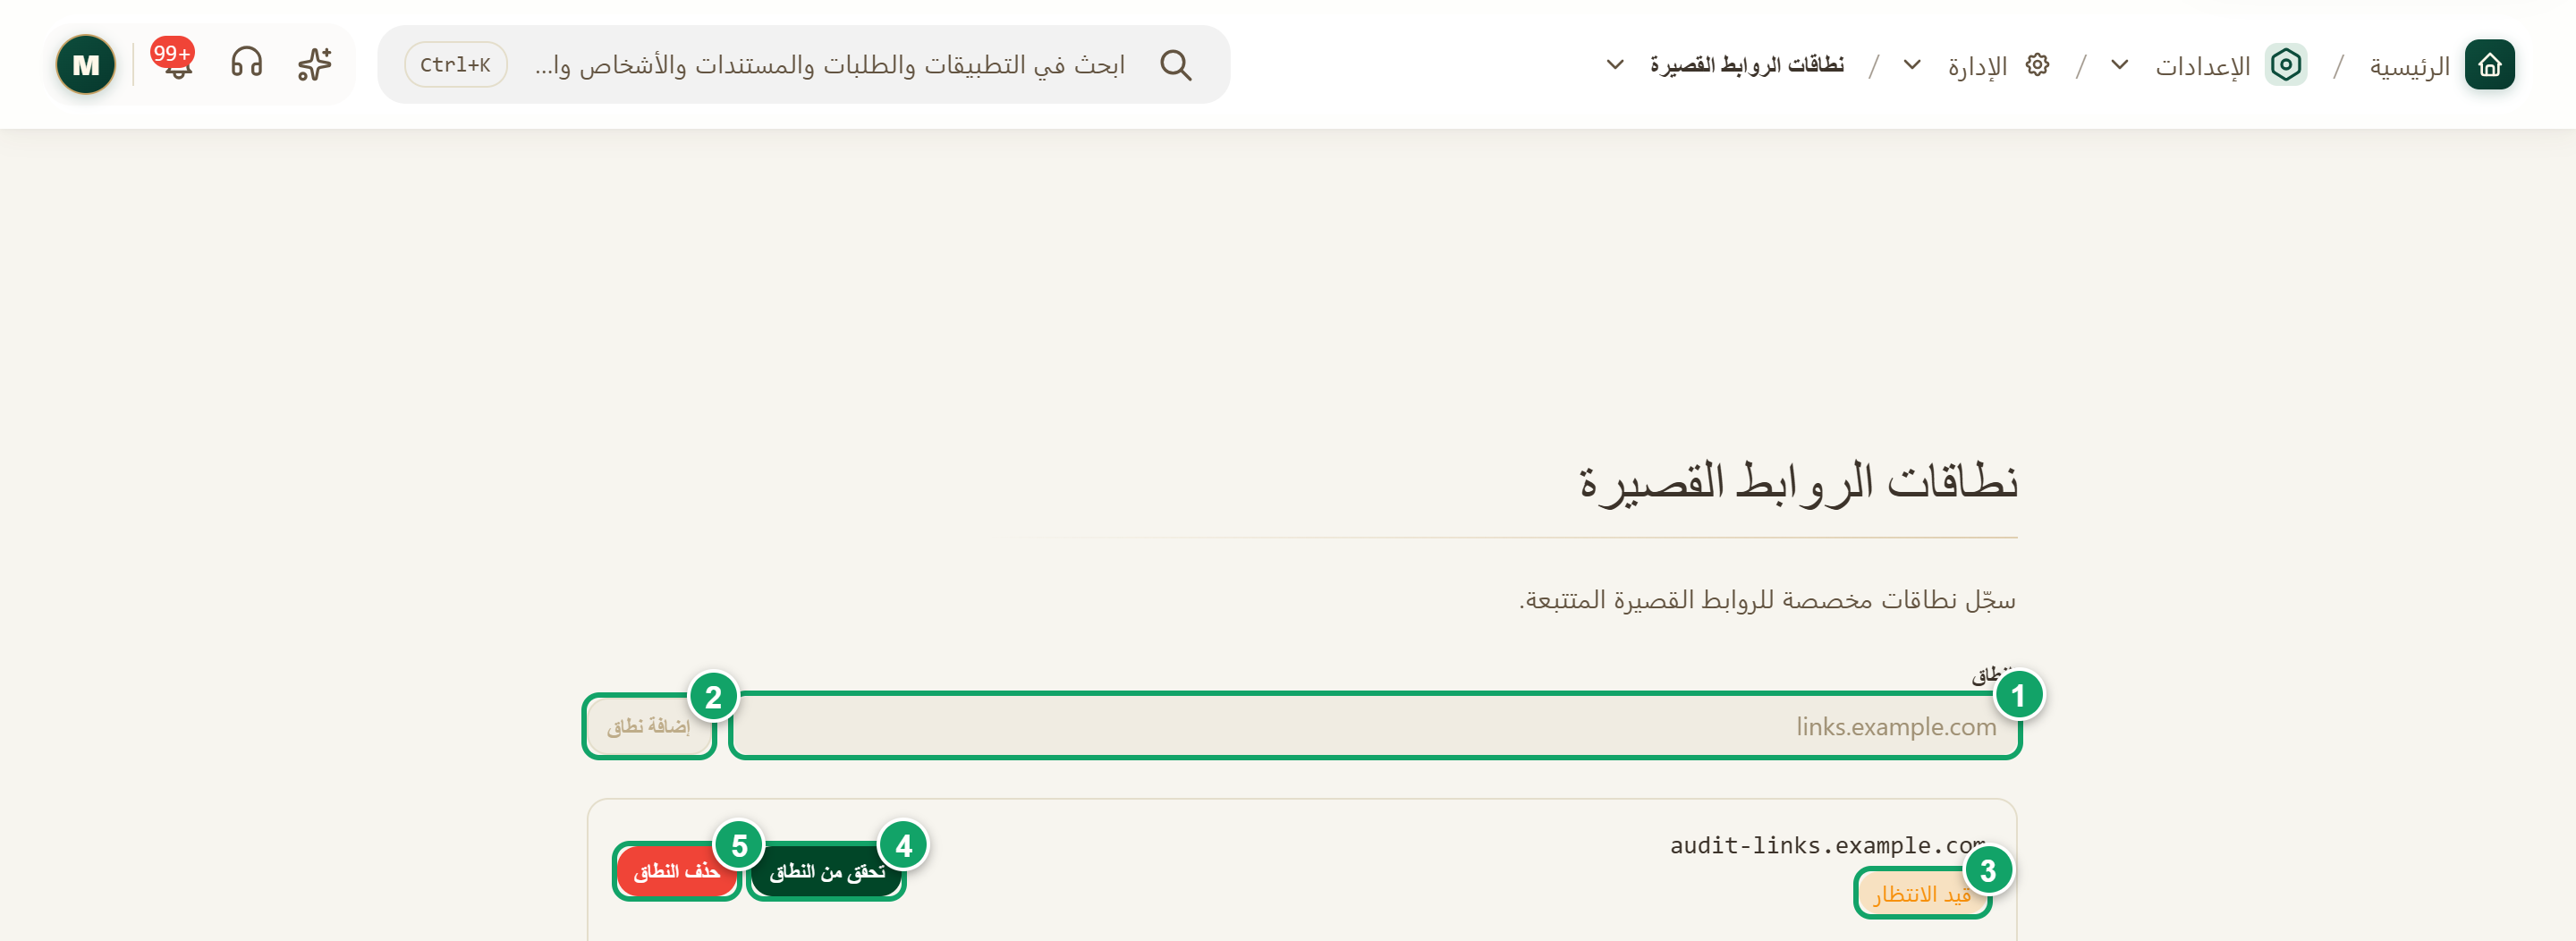
\includegraphics[width=0.95\linewidth,height=0.72\textheight,keepaspectratio]{figures/screens/ch08-short-links-ar.png}
\caption{نطاق روابط قصيرة قيد الانتظار}
\label{fig:settings-short-links}
\shotnote{تعرض الصورة نطاق اختبار لم يكتمل تحققه. توقفت الصورة قبل جدول السجلات لأن أول صف فيه يحمل قيمة تحقق خاصة، وشكل الجدول مشروح في صفحة نطاقات البريد. ① حقل «النطاق». ② «إضافة نطاق». ③ حالة النطاق. ④ «تحقق من النطاق». ⑤ «حذف النطاق».}
\end{figure}

\begin{table}[H]
\centering
\caption{ماذا تقرأ في نطاقات الروابط القصيرة؟}
\label{tab:settings-short-links-fields}
\begin{tabularx}{\linewidth}{R{4.2cm} Y}
\rcHeaderRow
\thh{البيان} & \thh{ماذا يعني؟}\\
«النطاق» & النطاق الفرعي الذي تخصصه للروابط.\\
سجل \en{TXT} & يثبت أنك تملك النطاق، وهو السجل الذي يفحصه زر التحقق.\\
سجل \en{CNAME} & يوجّه النطاق إلى العنوان الذي تعرضه الصفحة، حتى تعمل الروابط عند فتحها.\\
حالة النطاق & «قيد الانتظار» أو «نشط» أو «خطأ»، وتظهر «معطل» بعد حذف نطاق.\\
\end{tabularx}
\end{table}

\begin{enumerate}
\item افتح «الإعدادات»، ثم «نطاقات الروابط القصيرة».
\item اكتب النطاق، ثم اضغط «إضافة نطاق».
\item أضف السجلين الظاهرين في «سجلات \en{DNS}» عند مزوّد النطاق.
\item اضغط «تحقق من النطاق».
\end{enumerate}

\textbf{تحقق:} تصبح الحالة «نشط»، وتظهر الحالة «صالح» بجوار السجلين. أنشئ بعد ذلك رابطاً قصيراً وافتحه؛ فالتحقق لا يفحص سجل \en{CNAME}، وقد لا يعمل الرابط إذا كان هذا السجل ناقصاً.

\clearpage
\section{حسابات واتساب}
\label{sec:settings-feature-whatsapp}

تربط هذه الصفحة أرقام واتساب بالمؤسسة، لتظهر محادثاتها داخل الدردشة في النظام. يشبه الربط فتح واتساب على جهاز إضافي: يبقى الرقم على هاتفك، ويتصل به النظام كجهاز مرتبط. والحساب الشخصي يخص عضواً واحداً، أما الحساب المشترك فيخص فريقاً.

تختلف هذه الحسابات عن «واتساب · الرقم الرسمي» في صفحة الرسائل (\ref{sec:settings-feature-messages})؛ فذلك الرقم ترسل منه رسائل المتعاملين، أما هنا فالأرقام للمحادثات. تعرض الصفحة الحسابات التي يحق لك رؤيتها، ولا يظهر زر الربط إلا لمن يملك صلاحية إنشاء حساب. وتعود إلى الصفحة عندما ينقطع حساب عن الدردشة.

\begin{rcnote}[مثال: شركة الأفق]
يربط مسؤول النظام رقم فرع حلب بوصفه حساباً مشتركاً باسم واضح، لتتابع سارة الخطيب وعمر حداد محادثاته. وعندما يتوقف وصول الرسائل، يفتح الصفحة ويراجع البطاقة عند ④ ثم حالة الحساب في الجدول.
\end{rcnote}
\begin{figure}[H]
\centering
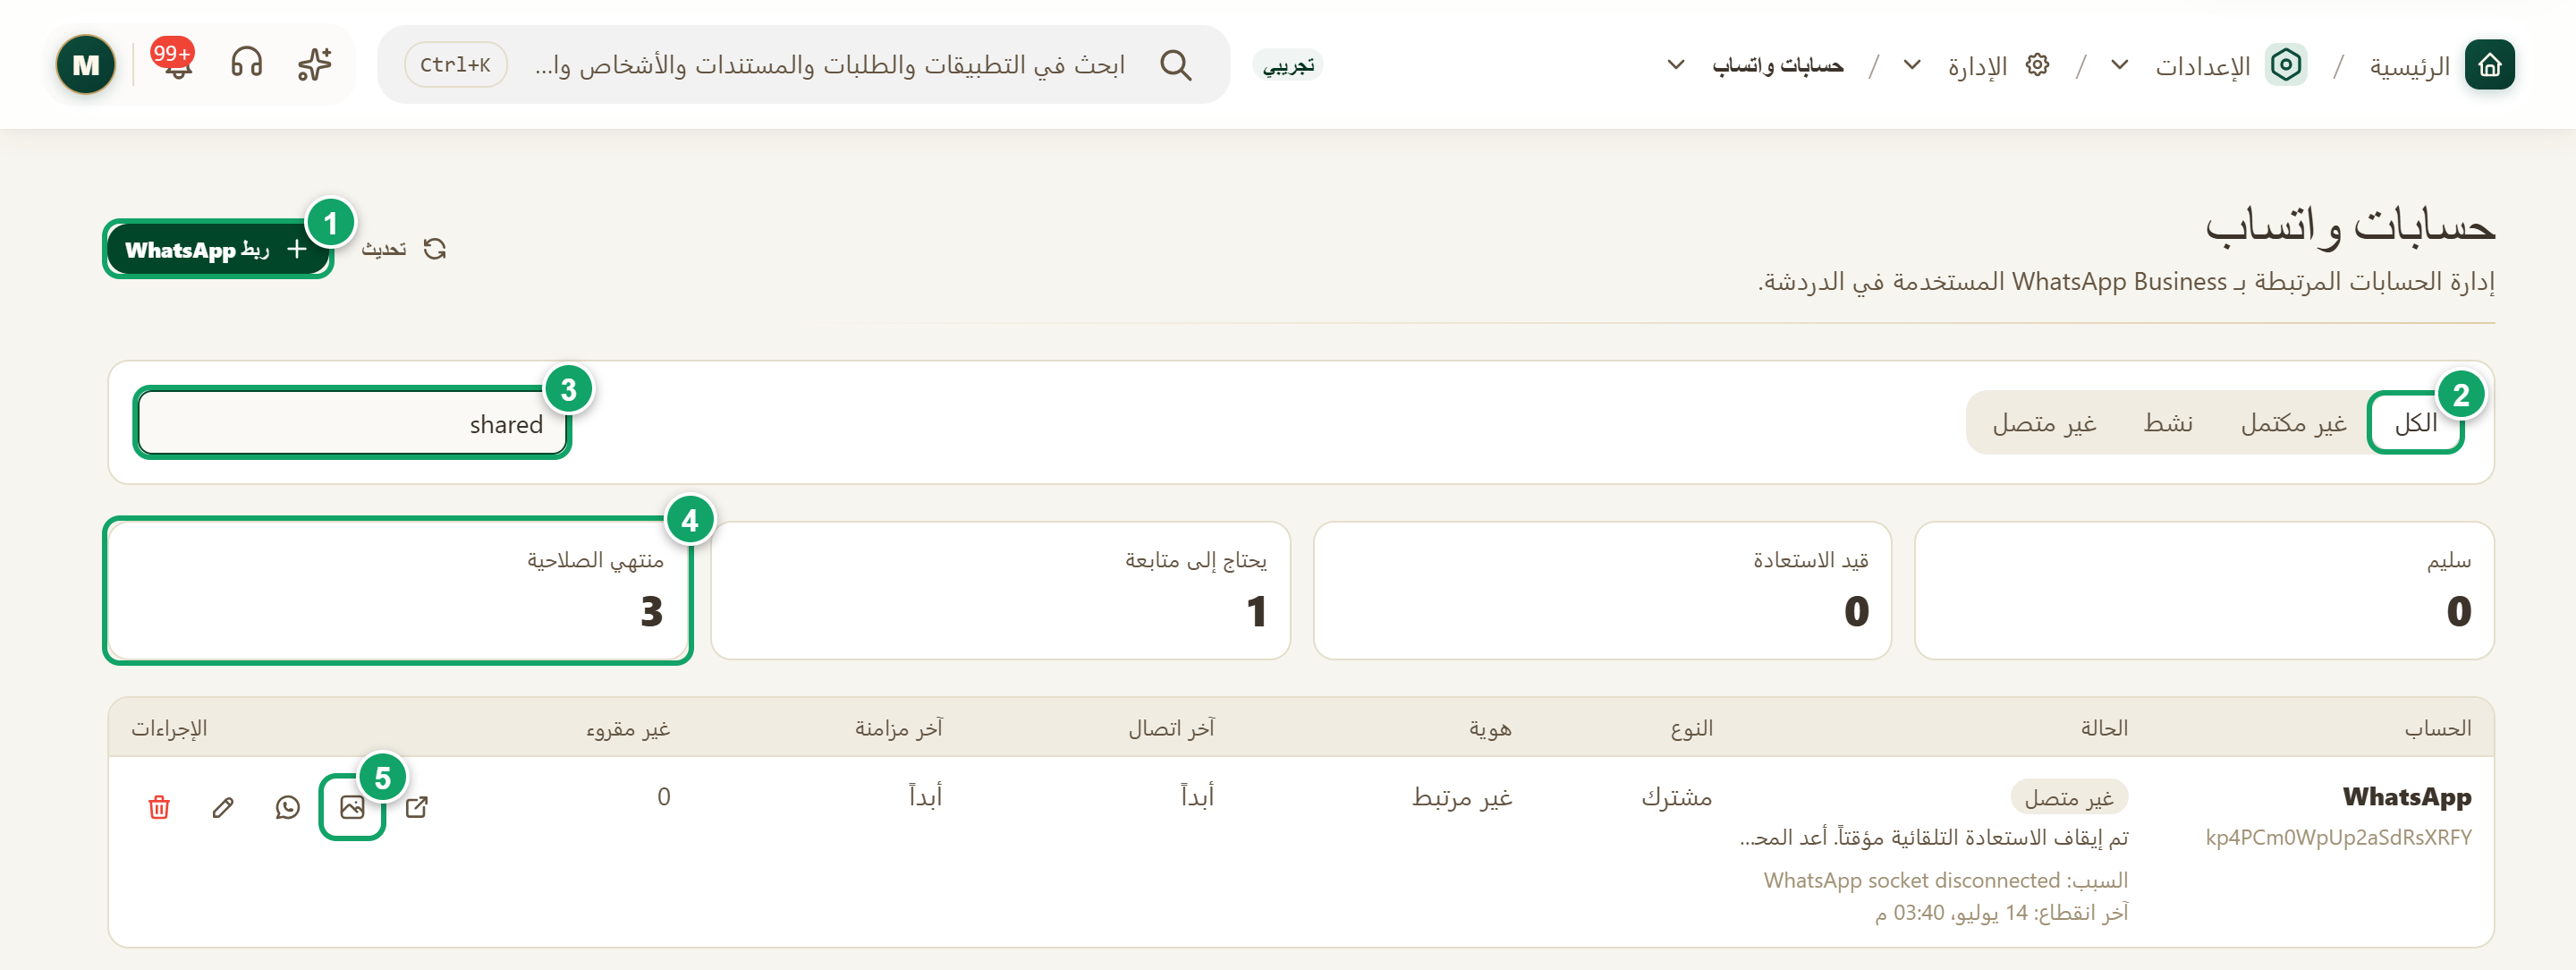
\includegraphics[width=0.95\linewidth,height=0.72\textheight,keepaspectratio]{figures/screens/ch08-whatsapp-ar.png}
\caption{قائمة حسابات واتساب}
\label{fig:settings-whatsapp}
\shotnote{تجمع البطاقات صحة الحسابات كلها، بينما يشرح الجدول حالة كل حساب وسبب انقطاعه. طُبّق البحث في الصورة ليظهر الحساب المشترك فقط، حتى لا تظهر أرقام هواتف شخصية، والبطاقات تحسب جميع الحسابات. ① «ربط \en{WhatsApp}». ② «الكل»: مع «غير مكتمل» و«نشط» و«غير متصل» لتصفية القائمة. ③ حقل البحث. ④ «منتهي الصلاحية»: حسابات تحتاج إلى إعادة ربط. ⑤ «حالة الوسائط»: تعرض حالة الصور والملفات وما فشل تنزيله.}
\end{figure}

\begin{figure}[H]
\centering
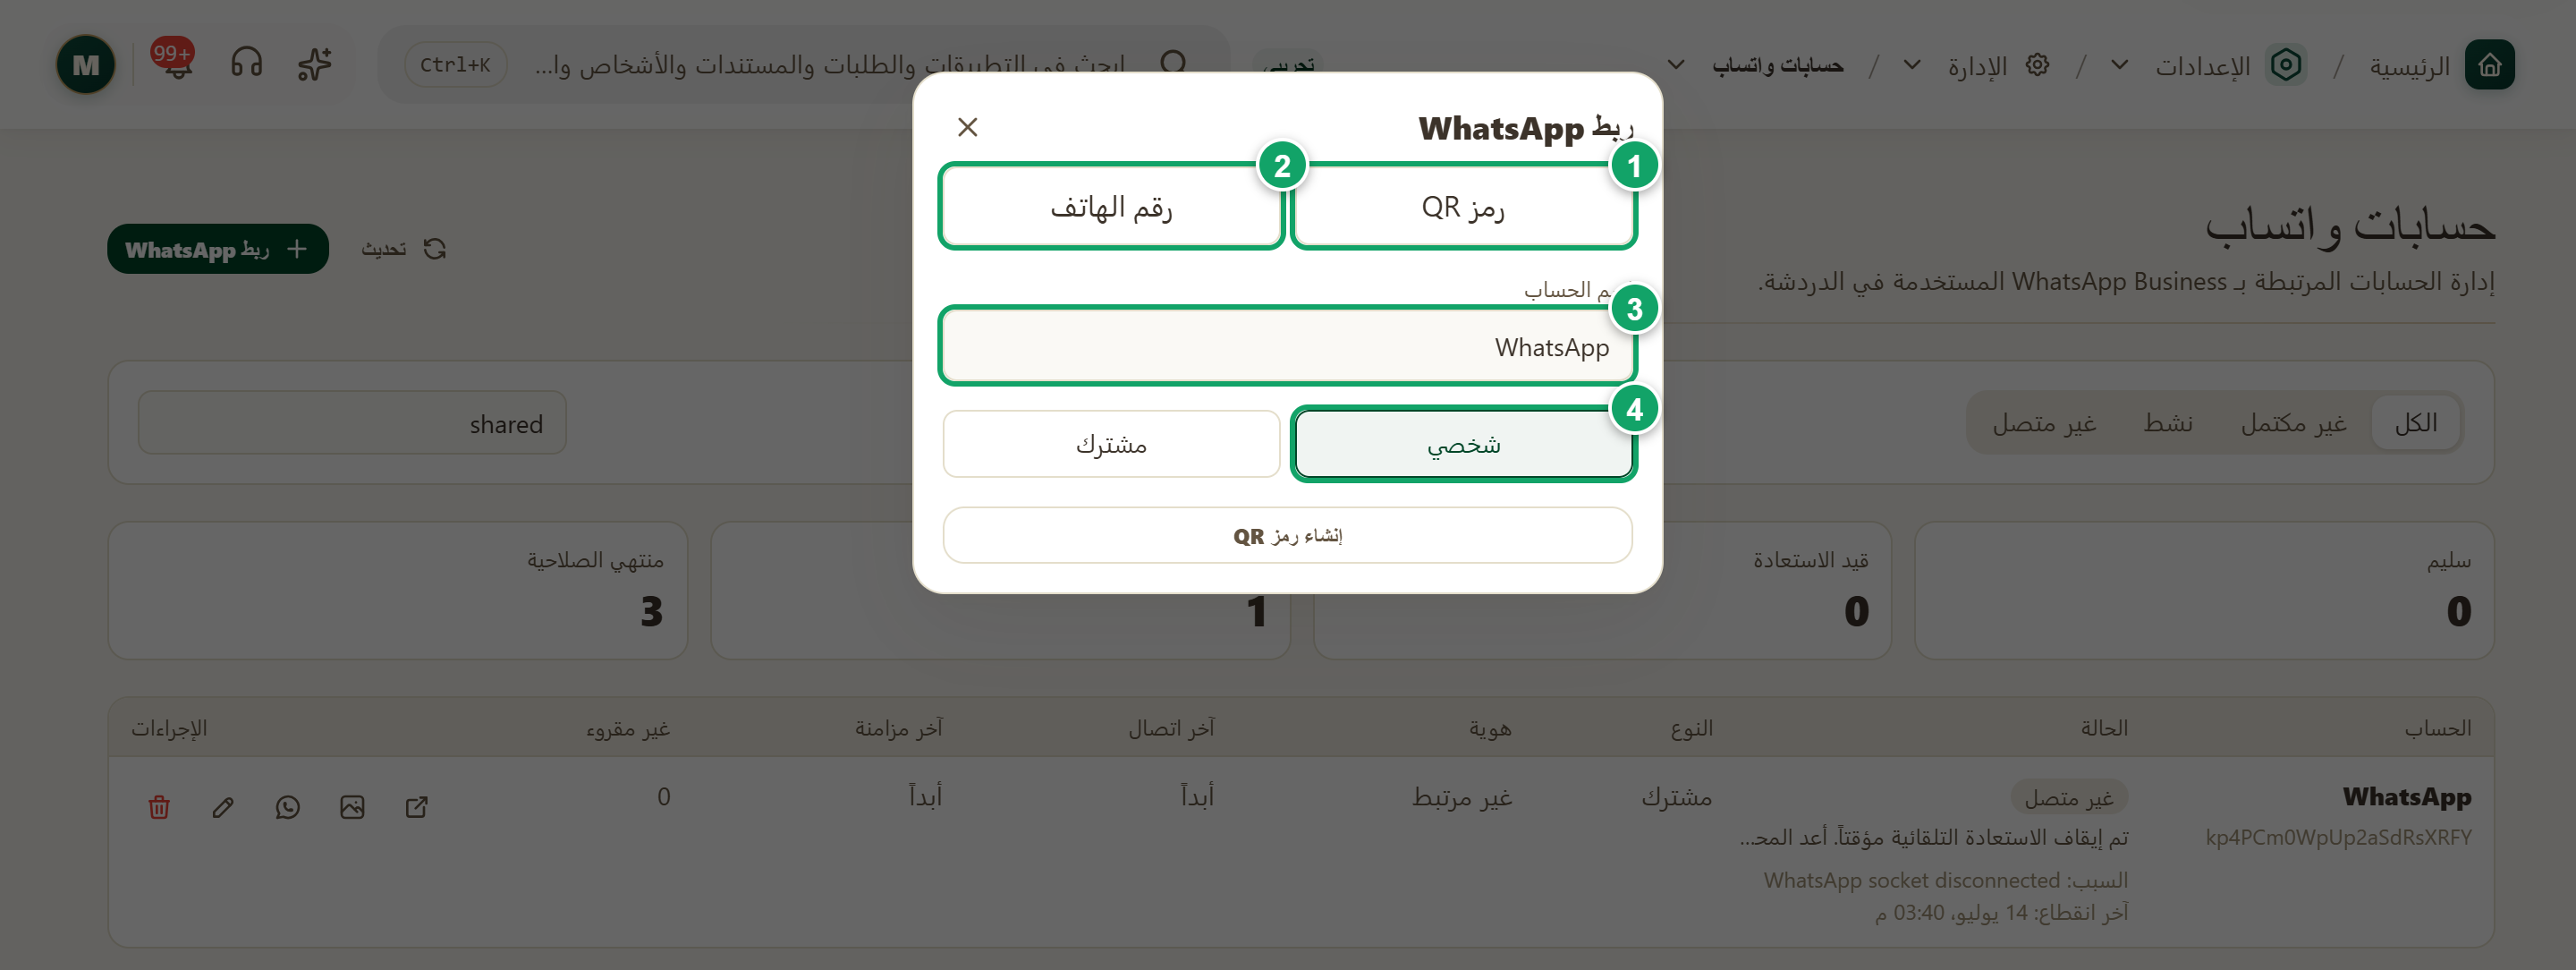
\includegraphics[width=0.95\linewidth,height=0.72\textheight,keepaspectratio]{figures/screens/ch08-whatsapp-link-ar.png}
\caption{نافذة ربط واتساب}
\label{fig:settings-whatsapp-link}
\shotnote{تعرض الصورة النافذة قبل بدء الربط، ولم يُنشأ أي حساب. لا يبدأ الربط إلا بعد الضغط على الزر أسفل النافذة، وعندها يظهر رمز تنتهي صلاحيته خلال وقت قصير. ① «رمز \en{QR}»: تمسحه بالهاتف. ② «رقم الهاتف»: تحصل به على رمز ربط تكتبه في واتساب. ③ «اسم الحساب». ④ «شخصي»، وبجواره «مشترك»: نوع الحساب.}
\end{figure}

\begin{table}[H]
\centering
\caption{ماذا تسجل وتقرأ في حسابات واتساب؟}
\label{tab:settings-whatsapp-fields}
\begin{tabularx}{\linewidth}{R{4.2cm} Y}
\rcHeaderRow
\thh{البيان} & \thh{ماذا يعني؟}\\
عند الربط & طريقة الربط، و«اسم الحساب»، ونوعه «شخصي» أو «مشترك».\\
البطاقات & «سليم»، و«قيد الاستعادة»، و«يحتاج إلى متابعة»، و«منتهي الصلاحية».\\
أعمدة الجدول & «الحساب»، و«الحالة» مع سبب الانقطاع، و«النوع»، و«هوية» وهو الرقم المرتبط، و«آخر اتصال»، و«آخر مزامنة»، و«غير مقروء».\\
الإجراءات & «فتح في الدردشة»، و«حالة الوسائط»، و«ربط الحساب»، و«إعادة المحاولة الآن»، و«فصل الحساب»، و«إعادة تسمية الحساب»، و«حذف الحساب». تظهر بحسب حالة الحساب وصلاحيتك.\\
\end{tabularx}
\end{table}

\begin{enumerate}
\item افتح «الإعدادات»، ثم «حسابات واتساب»، واضغط «ربط \en{WhatsApp}».
\item اختر «رمز \en{QR}» أو «رقم الهاتف».
\item اكتب «اسم الحساب»، واختر «شخصي» أو «مشترك».
\item بطريقة الرمز، اضغط «إنشاء رمز \en{QR}» ثم امسحه من «الأجهزة المرتبطة» في واتساب على الهاتف.
\item بطريقة الهاتف، اكتب الرقم مع رمز الدولة واضغط «الحصول على رمز الربط»، ثم أدخله في واتساب. يمكنك طلب رمز واحد كل دقيقة.
\end{enumerate}

\textbf{تحقق:} تُغلق النافذة، ويظهر الحساب في الجدول بحالة «نشط»، ويفتحه زر «فتح في الدردشة». إذا ظهرت «يلزم إعادة الربط» فاستخدم «ربط الحساب» من جديد. أما «حذف الحساب» فيطلب تأكيداً، ويفصل الجلسة النشطة أولاً.
